\documentclass[dp.tex]{subfiles}
\begin{document}
\chapter{Aplikace}

V rámci této diplomové práce byla vytvořena aplikace umožňující uživateli snadné provádění testů a analýz uvedených v kapitole~\ref{chap:denotacni_analyza}. Aplikace je tvořena dvěma moduly:
\begin{itemize}
\item knihovnou obstarávající analýzu textů,
\item modulem obsahujícím grafické uživatelské rozhraní -- \acrshort{gui}.
\end{itemize}

Oba moduly jsou naprogramovány v programovacím jazyce Java. Pro spuštění aplikace je proto potřeba nejprve nainstalovat běhové prostředí Java Virtual Machine \footnote{Dostupné z \url {https://java.com/en/download}}. Součástí přílohy této diplomové práce je CD, na kterém je mimo jiné i spustitelná verze aplikace ve formátu JAR.

Velkou výhodu Javy, jak napovídá i její motto \enq{write once, run anywhere}, je její multiplatformnost. To znamená, že v Javě napsaná aplikace je bez úprav spustitelná na všech \mbox{platformách}, pro něž je dostupná Java Virtual Machine. 

\section{Architektura aplikace}

Na začátku vývoje bylo třeba zvolit architekturu budoucí aplikace. Po předešlých zkušenostech z~oblasti vývoje softwaru jsem se rozhodl pro dva relativně nezávislé moduly, neboť čím je program jednodušší, tím méně je náchylný k chybám. 

Prvním z těchto modulů měla být knihovna, která bude provádět samotnou analýzu textu. Tato knihovna musela být z důvodu co nejvyšší spolehlivosti důkladně otestována. Dalšími požadavky byly:
\begin{itemize}
\item rychlost,
\item multiplatformnost,
\item snadná rozšiřitelnost (např. v rámci jiné závěrečné práce).
\end{itemize}

Druhý modul měl tuto knihovnu využívat a poskytnout k ní uživatelsky přívětivé grafické rozhraní (tzv. \acrshort{gui}). Grafické rozhraní mělo umožnit uživateli otevřít textový soubor (případně více souborů), provést na něm za pomoci modulu knihovny požadovanou analýzu a zobrazit její výsledky. Důležitým požadavkem na modul grafického rozhraní byla možnost exportu vstupních dat do souboru \acrshort{csv}. 

V rámci tohoto modulu pro mě zůstala stěžejní multiplatformnost a snadná rozšiřitelnost. Vzhledem k tomu, že cílem bylo vytvořit jednoduchý frontend \footnote{Frontend je software poskytující uživatelské rozhraní k jiným nástrojům. Samotný frontend žádnou činnost neprovádí, k práci jsou využívány nástroje, k nimž zprostředkovává přístup.}, nepředpokládal jsem, že by aplikace mohla být pomalá. Od automatizovaného testování jsem upustil, počítal jsem pouze s~testováním uživatelským.

Vzhledem k požadavkům (multiplatformnost obou modulů, rychlost modulu knihovny) sestávala moje prvotní představa z modulu knihovny napsaném v jazyce C (případně C++) a modulu uživatelského rozhraní napsaném v některém vyšším programovacím jazyce, přičemž jsem uvažoval zejména o interpretovaných jazycích jako Python či Ruby. 

Postupně jsem však od této idei upustil a to z následujících důvodů:
\begin{enumerate}
\item Jazyk C (resp. C++) je jazyk kompilovaný. Modul knihovny by musel být pro každou cílovou platformu zkompilován samostatně.
\item Jazyky uvažované pro vývoj modulu \acrshort{gui} (Ruby, Python, \ldots) vyžadují běhové prostředí -- interpret. Ten není standardní součástí operačního systému.
\item Rychlost vývoje:
	\begin{enumerate}
	\item Vývoj v C/C++ je obecně pomalejší oproti vývoji ve vyšším programovacím jazyce. 
	\item Předpokládal jsem, že při vývoji modulu uživatelského rozhraní nastane potřeba modul knihovny modifikovat. Každá taková změna by si vyžádala spuštění vývojového prostředí pro daný jazyk, modifikaci kódu, kompilaci.
	\end{enumerate}
\end{enumerate}

Po zavrhnutí výše popsaného návrhu jsem se rozhodl oba moduly naprogramovat v jednom jazyce. To znamenalo zvolit takový jazyk, který umožní napsat jak dostatečně rychlou a otestovatelnou knihovnu, tak vytvořit grafické uživatelské rozhraní. Ve výběru zůstaly dříve zmíněné jazyky Python a Ruby a přibyly do něj jazyky C\# (respektive Mono) a Java.

Vzhledem ke svým zkušenostem s jednotlivými jazyky jsem se nakonec rozhodl pro implementaci v jazyce Java, který splnil veškeré požadavky. 

\section{Knihovna \texttt{compLing}}

Modul knihovny jsem pojmenoval \enquote{compLing}. Název vychází z anglického \enquote{\textbf{comp}utational \textbf{ling}uistics}, což je označení pro matematickou lingvistiku. Knihovna implementuje analýzy textu popsané v kapitole \ref{chap:denotacni_analyza}. 

\sloppy
K vytvoření objektu knihovny se používá jedna statická metoda \texttt{ CompLing\allowbreak\#getInstance(String)}, jejímž parametrem je text, který má být analyzován. Tento text nesmí být hodnoty \texttt{null}. Třída \texttt{CompLing} obsahuje dvě vnitřní třídy:
\begin{enumerate}
%	\item \texttt{GeneralAnalysis},;
	\item \texttt{PoemAnalysis}.
\end{enumerate}

Tyto třídy zapouzdřují příbuzné typy analýz. Třída \texttt{GeneralAnalysis} poskytuje přístup k~analýze četnosti znaků (metodou \texttt{ICharacterFrequency characterFrequency()}) a slov (metodou \texttt{IWordFrequency wordFrequency()}). 

\sloppy
Třída \texttt{PoemAnalysis} umožňuje přístup k výsledkům analýz agregace (metoda \texttt{IAggregation aggregation()}), aliterace (metoda \texttt{IAlliteration alliteration()}), asonance (metoda \texttt{IAssonance assonance(String[])}) a k denotační analýze (metoda \texttt{IDenotation denotationAnalysis()}).

Všechny metody mají jako návratový typ deklarovaná rozhraní. To umožňuje změnit implementaci jednotlivých analýz beze změny \acrshort{api} knihovny. I knihovna \texttt{CompLing} je pomocí rozhraní odstíněna od konkrétních implementací jednotlivých analýz. Obojí je znázorněno v~diagramu tříd na obrázku \ref{fig:compling-core-class}:

\begin{figure}[h!]
	\centering
	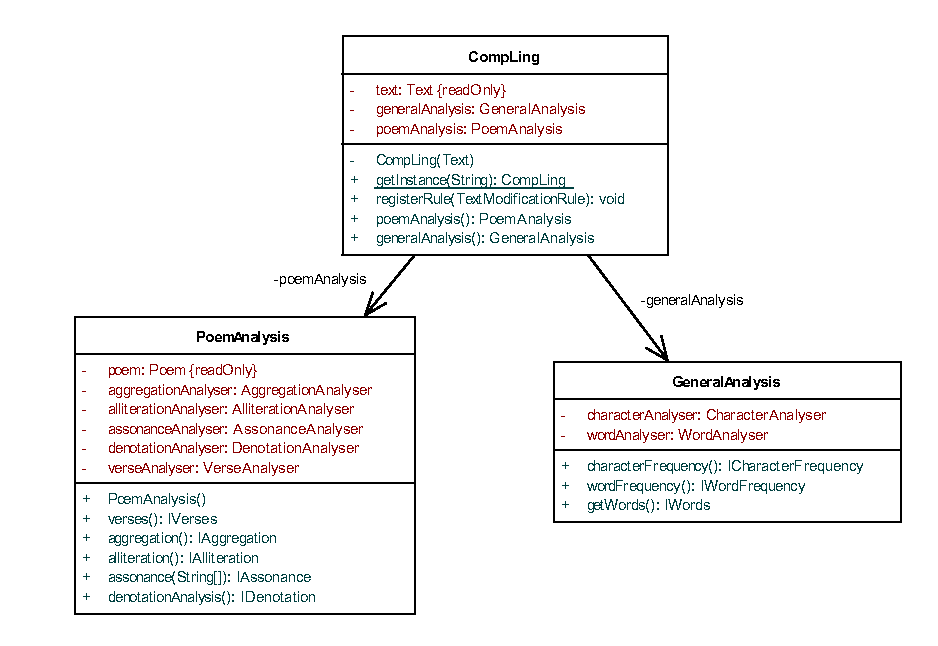
\includegraphics[max width=\textwidth,keepaspectratio=true]{imgs-60-aplikace/compLing-class-diagram.pdf}
	\caption{Diagram tříd jádra knihovny \texttt{compLing}.}
	\label{fig:compling-core-class}
\end{figure}

\section{Grafické uživatelské rozhraní}

Modul grafického uživatelského rozhraní vznikl jako nutná nadstavba nad knihovnou \texttt{compLing}, neboť knihovna sama neposkytuje žádnou jinou možnost použití (např. pomocí příkazové řádky) než \acrshort{api} a je tedy nutné začlenit ji do jiného softwarového modulu.

Cílem bylo vytvořit co možná nejjednodušší rozhraní, které uživateli umožní otevřít libovolný počet textů a následně nad těmito texty provádět analýzy podporované knihovnou \texttt{compLing}. Uživatelské rozhraní programu s 18 otevřenými překlady básně Havran je zobrazeno na následujícím obrázku:

\begin{figure}[H]
	\centering
	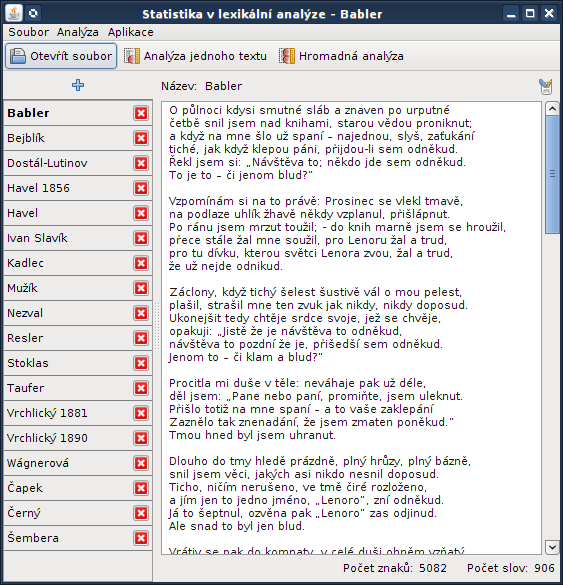
\includegraphics[max width=\textwidth,keepaspectratio=true] {imgs-60-aplikace/gui-main-window}
	\caption{Hlavní okno programu s otevřenými překlady básně Havran.}

	\medskip % induce some separation between caption and explanatory material
	\begin{minipage}{\textwidth} % choose width suitably
		\begin{center}
			{\footnotesize \textit{Pozn.: v závislosti na operačním systému se vzhled může lišit.}\par}
		\end{center}
	\end{minipage}
		
	\label{fig:gui-main-window}
\end{figure}

Hlavní okno je rozděleno do čtyř částí:

\begin{enumerate}
	\item menu,
	\item panel nástrojů
	\item panely otevřených textů,
	\item aktuální text.
\end{enumerate}

Menu aplikace obsahuje tři položky -- \menu{Soubor}, \menu{Analýza} a \menu{Aplikace}. V menu \menu{Soubor} se nacházejí položky pro vytvoření nového prázdného panelu, otevření souboru, uložení aktuálního textu a ukončení aplikace. Menu \menu{Analýza} zpřístupňuje jednotlivé type analýz (kvantitativní, fonické, denotační). V případě, že není otevřen žádný text, je tato položka neaktivní. V menu \menu{Aplikace} se skrývají dvě položky --- \menu{Nastavení} a \menu{O aplikaci}. Položka \menu{Nastavení} vyvolá dialog, který umožňuje upravit velikost písma v aplikaci a změnit vzhled grafů, jež jsou vytvořeny při denotační analýze.

Panel nástrojů poskytuje rychlý přístup k nejčastěji využívaným funkcím. Těmi jsou otevírání textů, analýza aktuálního textu a analýza všech otevřených textů. Po kliknutí na tlačítko \menu{Analýza jednoho textu} nebo \menu{Hromadná analýza} je zobrazeno menu pro výběr konkrétního typu analýzy. Obě tato tlačítka jsou neaktivní, není-li otevřen žádný text.

Pod panelem nástrojů vlevo jsou ve sloupci umístěny panely pro otevřené texty. Nad nimi se nachází tlačítko pro vytvoření nového prázdného panelu. Po kliknutí pravým tlačítkem myši na panel se zobrazí kontextové menu, pomocí kterého je možné panel přejmenovat, uložit, znovu načíst nebo uzavřít.

Napravo od těchto panelů je zobrazen právě aktivní text. Nad i pod textem je umístěn informační panel. Vrchní zobrazuje jméno aktivního textu. Kliknutím na tlačítko vpravo (ikonka tužky) je možné text přejmenovat. Na panelu umístěném pod textem je zobrazena informace o délce aktuálního textu, a to jak v počtu znaků, tak v počtu slov.

\section{Práce s aplikací}

Tato sekce obsahuje popis funkcí aplikace včetně ukázek, jak tyto funkce využívat. Přestože se aplikace snaží být co nejvíce uživatelsky přívětivá, ne všechny funkce mohou být na první pohled zcela zřejmé.

\subsection{Spuštění aplikace}

Spustitelná aplikace je součástí elektronické přílohy této diplomové práce. Na přiloženém CD je umístěn soubor \texttt{CompLingGui.jar}. Tento soubor je vhodné zkopírovat z CD na pevný disk počítače, na kterém má být aplikace spuštěna. Aplikaci lze spustit poklepáním na ikonu souboru \texttt{CompLingGui.jar}. Nastat mohou tři situace:

\begin{enumerate}
\item aplikace se spustí,
\item spustí se jiná aplikace (typicky archivační program, např. WinZip),
\item operační systém nemá pro soubor s příponou \texttt{jar} nastavenu žádnou asociaci a zobrazí dialog:
\end{enumerate}

\raggedbottom

\begin{figure}[H]
	\centering
	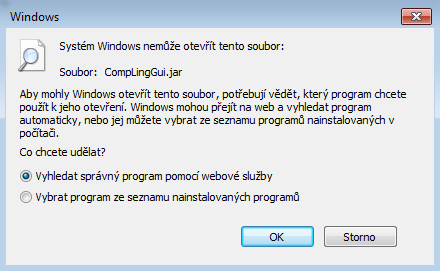
\includegraphics[max width=\textwidth,keepaspectratio=true] {imgs-60-aplikace/no-association}
	\caption{Žádná asociace pro soubory typu \texttt{jar} nenastavena.}
	\label{fig:no-association}
\end{figure}

V případě, že nastane první situace, je vše v pořádku. V opačném případě je třeba operačnímu systému říci, že má soubory typu \texttt{jar} spouštět programem \texttt{Java}. Ten již může být na počítači nainstalovaný z dřívějška, ale může se stát, že vůbec nainstalovaný není.

Pokud nastala druhá situace, tj. spustil se jiný program, než ten z obrázku ~\ref{fig:gui-main-window}, uzavřete jej, zkuste na ikonku souboru \texttt{CompLingGui.jar} kliknout pravým tlačítkem myši. Objeví se kontextové menu. Pokud menu obsahuje položku \menu{Otevřít v programu $\kern 10pt\triangleright$}, a v podmenu této položky je na výběr \menu{Java(TM)}, zvolte tuto možnost. Nyní by se měla aplikace spustit.

V případě, že Java nainstalovaná není, je třeba ji nejprve stáhnou z internetových stránek \url{https://java.com/en/download/} a poté nainstalovat. Instalátor by měl sám zajistit asociaci souborů typu \texttt{jar} s Javou. Po skončení instalace je vhodné restartovat počítač. Po restartu je možné aplikaci spustit dvojklikem na ikonu souboru \texttt{CompLingGui}.

\subsection{Práce s texty}

Po spuštění je zobrazeno hlavní okno grafického uživatelského rozhraní aplikace. Protože zatím není otevřen žádný text, je funkcionalita programu omezena o možnost provádění analýz. Pro to, aby se analyzování zpřístupnilo, je třeba vytvořit nový nebo otevřít existující text.

Pro vytvoření nového prázdného textu je třeba pomocí tlačítka \menu{\ding{58}} nejprve vytvořit nový panel (eventuálně je možné pro vytvoření panelu použít menu \menu[,]{Soubor,Nový prázdný panel}). Aplikace poté vyzve k zadání jména pro nový text. Jméno textu nemůže zůstat prázdné. Do \mbox{nového} panelu je možné vepsat nebo vložit vlastní text. Ten může být uložen buď pomocí menu \menu[,]{Soubor,Uložit}, nebo přes kontextové menu, které je vyvoláno po kliknutí pravým tlačítkem myši na panel.

Další možností je otevřít již existující textový soubor (soubor s příponou \texttt{txt}). To je možné provést buď pomocí menu \menu[,]{Soubor,Otevřít}, nebo tlačítkem \menu{Otevřít soubor} na panelu nástrojů. Po zvolení jedné z možností se zobrazí dialog pro výběr souboru. Je možné otevřít více textů najednou označením více souborů pomocí klávesy \keys{\ctrl} a levého tlačítka myši. Pro každý z~otevřených souborů je vytvořen nový panel, který je pojmenován stejně jako otevíraný soubor.

Je-li text změněn, objeví se za jeho jménem na panelu znak \texttt{*}. Změněný text je možné uložit (buď v kontextovém menu vyvolaném kliknutím pravého tlačítka myši na panel nebo v menu \menu{Soubor}), případně jej lze, je-li text načten ze souboru, znovu načíst a vrátit jej tak do původní podoby. Tato možnost je přístupná přes kontextové menu příslušného panelu (\menu[,]{klik pravým tlačítkem na panel,Nahrát znovu}).

Otevřené texty je možné uzavřít buď kliknutím na uzavírací tlačítko \menu{\ding{54}}, které se nachází na panelu vpravo, nebo přes \menu[,]{kontextové menu panelu, Zavřít}. Aplikace zobrazí varování v případě, že byl text před uzavřením změněn a není uložen. Stejně tak je varování zobrazeno, pokud je aplikace ukončena a jsou v ní otevřené texty, které byly změněny a dosud nejsou uloženy.

\subsection{Analyzování textu obecně}

Analýza textu vyžaduje, aby byl otevřen alespoň jeden panel s textem. Tím se zpřístupní menu \menu{Analýza} i tlačítka pro rychlý přístup \keys{Analýza jednoho textu} a \keys{Hromadná analýza}.  Některé analýzy je možno provádět jak nad jedním tak nad všemi otevřenými texty. Jiné typy analýz (aliterace, denotační analýza) je možné vykonat pouze nad jedním textem, některé naopak vyžadují více otevřených textů (asonance).

Je-li otevřen pouze jeden text, je hromadná analýza prováděna pouze nad jedním textem.

\subsection{Analýza četnosti znaků}
\label{chap:analyza-cetnosti-znaku}

Analýzu četnosti znaků je možné provést jak pro jeden tak pro všechny otevřené texty. V závislosti na množině analyzovaných textů je analýza četnosti znaků dostupná:
\begin{description}
  \item[Analýza jednoho textu] \hfill \\
	Přes menu \menu[,]{Analýza,Četnost znaků,Pro aktuální text} nebo přes tlačítko \menu[,]{Analýza jednoho textu,Četnost znaků}.
  \item[Analýza všech otevřených textů] \hfill \\
	Přes menu \menu[,]{Analýza,Četnost znaků,Pro všechny texty} nebo přes tlačítko \menu[,]{Hromadná analýza,Četnost znaků}.
\end{description}

Po zvolení požadovaného typu analýzy je zobrazen dialog, ve kterém je možné upřesnit nastavení:

\begin{figure}[H]
\centering
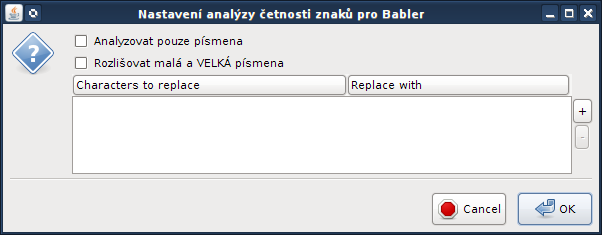
\includegraphics[max width=\textwidth,keepaspectratio=true]{imgs-60-aplikace/gui-character-analysis-dialog}
\caption{Nastavení analýzy četnosti znaků.}
\label{fig:gui-character-analysis-dialog}
\end{figure}

Dialog obsahuje dvě zaškrtávací políčka a tabulku pravidel, která mohou být aplikována na analyzované texty před samotnou analýzou. Pro názornost	budou funkce jednotlivých voleb demonstrovány na větě 

\begin{center}
\textit{\enquote{Pan Novák se chechtal 10$\times$ denně.}}
\end{center}

Pokud v dialogu není nic změněno, je text převeden na velká písmena a analyzovány jsou všechny znaky. Výsledkem analýzy je tabulka obsahující četnosti jednotlivých znaků:
\begin{table}[H]
\caption {Četnost znaků ve výchozím nastavení} 
\label{tab:title} 
\centering
	\begin{tabular}{|l|c|c|c|c|c|c|c|c|c|c|c|c|c|c|c|c|c|c|c|c|}


	\hline \textbf{Znak} & ' ' & N & E & A & C & H & D & L & Ě & O & . & Á & K & T & 1 & 0 & V & P & S & $\times$ \\ 
	\hline \textbf{Výskytů} & 5 & 4 & 3 & 2 & 2 & 2 & 1 & 1 & 1 & 1 & 1 & 1 & 1 & 1 & 1 & 1 & 1 & 1 & 1 & 1 \\ 
	\hline 
	\end{tabular} 
\end{table} 

Zaškrtnutím možnosti \enquote{Analyzova pouze písmena} budou z textu před analýzou odstraněny znaky, které nejsou písmeny (číslice, interpunkce, \ldots). Výsledná tabulka četností by tomto případě vypadala takto:
\begin{table}[H]
\caption {Četnost znaků s volbou \enquote{Analyzovat pouze písmena}} 
\label{tab:title} 
\centering
	\begin{tabular}{|l|c|c|c|c|c|c|c|c|c|c|c|c|c|c|c|c|c|}


	\hline \textbf{Znak} & N & E & A & C & H & D & T & V & P & S & L & Ě & O & Á & K  \\ 
	\hline \textbf{Výskytů} & 4 & 3 & 2 & 2 & 2 & 1 & 1 & 1 & 1 & 1 & 1 & 1 & 1 & 1 & 1 \\ 
	\hline 
	\end{tabular} 
\end{table} 

Další volbou je možnost \enquote{Rozlišovat malá a VELKÁ písmena}. Zaškrtnutím této volby nebude text před začátkem analýzy převeden na velká písmena, takže v tabulce četností budou zvlášť zobrazeny výskyty pro malá i velká písmena nalezená v textu:

\begin{table}[H]
\caption {Četnost znaků s volbou \enquote{Rozlišovat malá a VELKÁ písmena}} 
\label{tab:title} 
\centering
	\begin{tabular}{|l|c|c|c|c|c|c|c|c|c|c|c|c|c|c|c|c|c|c|c|c|c|}


	\hline \textbf{Znak} & ' ' & e & n & c & a & h & d & ě & o & N & l & . & k & á & v & 1 & 0 & t & s & P & $\times$ \\ 
	\hline \textbf{Výskytů} & 5 & 3 & 3 & 2 & 2 & 2 & 1 & 1 & 1 & 1 & 1 & 1 & 1 & 1 & 1 & 1 & 1 & 1 & 1 & 1 & 1 \\ 
	\hline 
	\end{tabular} 
\end{table} 

Tyto dvě volby je možné zkombinovat (tj. analyzovat pouze písmena a rozlišovat jejich velikost).

Další možností, jak ovlivnit analýzu, je definování pravidel. Pravidla je možné definovat po kliknutí na tlačítko \menu{\ding{58}} na pravém okraji okna. Objeví se nový dialog.

\begin{figure}[H]
\centering
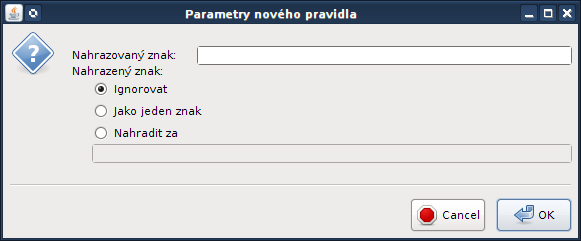
\includegraphics[max width=\textwidth,keepaspectratio=true]{imgs-60-aplikace/gui-character-analysis-rules-dialog}
\caption{Nastavení pravidel analýzy četnosti znaků.}
\label{fig:gui-character-analysis-rules-dialog}
\end{figure}

Pokud by analýza měla fungovat tak, že
\begin{itemize}
\item budou ignorovány mezery,
\item sousedící znaky \enquote{c} a \enquote{h} budou považovány za jedno písmeno \enquote{ch},
\item znak \enquote{$\times$} bude považován za písmeno \enquote{x},
\end{itemize}

je třeba vytvořit tato pravidla:

\begin{figure}[H]
\centering
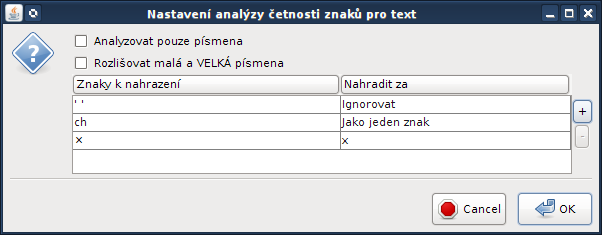
\includegraphics[max width=\textwidth,keepaspectratio=true]{imgs-60-aplikace/gui-character-analysis-dialog-with-rules}
\caption{Nastavení pravidel analýzy četnosti znaků.}
\label{fig:gui-character-analysis-dialog-with-rules}
\end{figure}

Výsledkem takto nastavené analýzy bude tato tabulka četnosti znaků:

\begin{table}[H]
\caption {Četnost znaků s aplikovanými pravidly} 
\label{tab:title} 
\centering
	\begin{tabular}{|l|c|c|c|c|c|c|c|c|c|c|c|c|c|c|c|c|c|c|c|c|c|}


	\hline \textbf{Znak} & N & E & A & CH & D & L & Ě & O & Á & K & T & 1 & 0 & V & P & S & x \\
	\hline \textbf{Výskytů} & 4 & 3 & 2 & 2 & 1 & 1 & 1 & 1 & 1 & 1 & 1 & 1 & 1 & 1 & 1 & 1 & 1 \\ 
	\hline 
	\end{tabular} 
\end{table} 

Výsledek analýzy je zobrazen v novém okně. Obsahuje informace o analýze, jako je seznam analyzovaných textů, počet všech znaků, počet unikátních znaků, nejčastěji se vyskytující znak a informaci o tom, zda je analyzovaný výběr se zvolenou směrodatnou odchylkou na základě Kubáčkova vzorce (\ref{eq:kubacek}, viz \cite[str.~22]{Wimmer2003}) reprezentativní:

\begin{equation}
\label{eq:kubacek}
N = \frac{1}{r^2} \prod_{x=1}^{k} p_x^{\frac{1}{k-1}},
\end{equation}
kde 
\begin{align*}
      p_x & \text{ je relativní frekvence výskytu entity $x$,}\\
      r   & \text{ je průměrná směrodatná odchylka odhadů $p_i$ (může být určena dopředu),}\\
      k   & \text{ je počet entit.}
\end{align*}   

Pod souhrnem se nachází tabulka četností znaků. Ta obsahuje jednak sloupec s relativními četnostmi každého znaku a jednak sloupec s absolutními četnostmi pro každý analyzovaný text. Tabulku je možné seřadit dle libovolného sloupce kliknutím na jeho název.

Výsledek analýzy dále obsahuje dva grafy. První z nich zobrazuje četnosti jednotlivých znaků. Výchozím typem grafu je graf koláčový. Po kliknutí levým tlačítkem se typ grafu změní na sloupcový, který zobrazuje absolutní četnosti výskytu znaků. Dalším kliknutím levým tlačítkem myši se změní zobrazované hodnoty z absolutních na relativní. Další kliknutím je opět zobrazen původní koláčový graf.

Druhý graf má smysl zejména při analýze více textů. Zobrazuje porovnání výskytů zvolených znaků v jednotlivých analyzovaných textech. Do srovnání je možné přidat všechny z~nalezených znaků.

\subsection{Analýza četnosti slov}

Stejně jako analýza četnosti znaků může být i analýza četnosti slov prováděna jak na jednom, tak více textech najednou. Analyzovat četnost slov lze buď z menu \menu[,]{Analýza,Analýza četnosti slov} nebo z nástrojového panelu pomocí tlačítek \menu[,]{Analýza jednoho textu}, případně \menu[,]{Hromadná analýza}.

Předtím než analýza začne, je možné nastavit její parametry pomocí dialogu \ref{fig:gui-word-analysis-dialog}:
\begin{figure}[H]
\centering
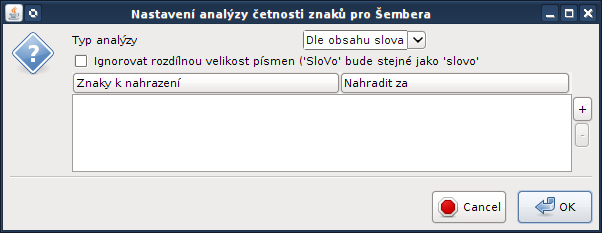
\includegraphics[max width=\textwidth,keepaspectratio=true]{imgs-60-aplikace/gui-word-analysis-dialog}
\caption{Nastavení analýzy četnosti slov.}
\label{fig:gui-word-analysis-dialog}
\end{figure}

Aplikace podporuje dva způsoby, jak počítat četnost slov:

\begin{enumerate}
\item dle obsahu slova (tedy dvě slova jsou stejná, pokud obsahují stejná písmena ve stejném pořadí),
\item dle délky slova (ve znacích).
\end{enumerate}

Způsob, který má být použit, je možné zvolit v nabídce \keys{Typ analýzy}. Další volbou je možnost ignorovat rozdílnou velikost písmen. Ve výchozím nastavení je tato volba vypnuta, což znamená, že například ve verši

\begin{verse}
\enquote{Sám a sám tak havran sedí,\ldots}
\begin{flushright}
\textit{(Havran ---překlad Rudolf Havel)}
\end{flushright}
\end{verse}

by slova \enquote{Sám} a \enquote{sám} byla brána jako dvě různá slova. Zaškrtnutím volby \keys{Ignorovat rozdílnou velikost písmen} bude text před analýzou převeden na malá písmena, takže obě slova budou považována za jedno. Tato volba nijak neovlivní výsledek v případě, že je jako typ analýzy zvolena analýza dle délky slova.

Poslední možností, jak ovlivnit výsledek analýzy četnosti znaků, je vytvoření pravidel podobných těm z kapitoly \hyperref[chap:analyza-cetnosti-znaku]{Analýza četnosti znaků}. Pravidla je možné vytvořit v dialogu, který se zobrazí po kliknutí na tlačítko \menu{\ding{58}}:

\begin{figure}[H]
\centering
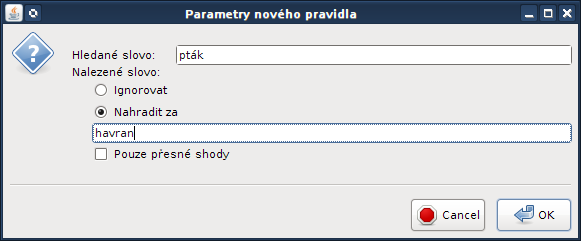
\includegraphics[max width=\textwidth,keepaspectratio=true]{imgs-60-aplikace/gui-word-analysis-rules-dialog}
\caption{Nastavení pravidel analýzy četnosti slov.}
\label{fig:gui-word-analysis-rules-dialog}
\end{figure}

Dialog umožňuje vytvoření pravidel dvou typů. Hledané slovo (\enquote{pták}) je možné buď ignorovat (tzn., že je při analýze přeskočeno a výsledcích se vůbec neobjeví), nebo nahradit \mbox{slovem} jiným. V tomto případě bude výskyt slova \enquote{pták} přičten k počtu výskytů slova \enquote{havran}.

Zaškrtávací tlačítko \keys{Pouze přesné shody} umožňuje ovlivnit, jak bude analýza probíhat v případě, že hledané slovo je prefixem právě analyzovaného slova (například slovo \enquote{\textbf{pták}u} \mbox{začíná} hledaným slovem \enquote{pták}). V případě, kdy nebude zaškrtnuto tlačítko \keys{Pouze přesné shody}, bude ve slově \enquote{\textbf{pták}u} část \enquote{pták} nahrazena slovem \enquote{havran}. Do zpracování analýzy tedy vstoupí slovo \enquote{\textbf{havran}u}. Pokud by byla zvolena volba \keys{Pouze přesné shody}, nebylo by nahrazení na slovo \enquote{ptáku} aplikováno a do analýzy by vstoupilo nezměněné slovo \enquote{ptáku}.


Výsledkem analýzy četnosti slov je report obsahující jednak souhrnné informace o analyzovaných textech a jednak detailní přehled zobrazený buď formou tabulky, nebo grafu. Souhrn obsahuje informace jako celkový počet nalezených slov, nejčastěji se vyskytující slovo (délka slova) atd. V reportu je dále uvedena tabulka četností jednotlivých slov (resp. jejich délek). Tato tabulka je ve výchozím stavu sbalena, což indikuje ikona za nadpisem \enquote{Tabulka četností výskytu slov} (příp. \enquote{Výskyt slov dle délky slova}):

\begin{figure}[H]
\centering

\includegraphics[max width=\textwidth,keepaspectratio=true]{imgs-60-aplikace/gui-toggle-healine}
\caption{Ikona rozbalitelných nadpisů ve stavu \enquote{sbaleno}}
\label{fig:gui-toggle-healine}
\end{figure}

Kliknutím na nadpis se tabulka rozbalí. Tabulku je možné řadit dle libovolného sloupce kliknutím levým tlačítkem myši na hlavičku příslušného sloupce.

V případě analýzy dle délky slova, je pod tabulkou četností zobrazena další tabulka, která přísluší k $\chi^2$ testu. Hypotéza $H_0$ tohoto testu zní \enquote{Rozdělení četností slov dle délky odpovídá Poissonovu rozdělení}. V tabulce jsou zobrazeny naměřené počty a četnosti daných délek spolu s jejich očekávanými hodnotami. Pod tabulkou je zobrazen výsledek testu na zvolené hladině významnosti včetně kritických hodnot. Hodnotu hladiny významnosti  $\alpha$ je možné změnit.

V reportu je dále zobrazen graf zastoupení jednotlivých slov (resp. délek slov). Výchozí je graf koláčový, který se kliknutím levým tlačítkem myši změní na graf sloupcový, v němž jsou zobrazeny absolutní četnosti výskytů. Dalším kliknutím se na osu $y$ vynesou relativní četnosti. Vzhledem k tomu, že slov v textu bývá obsaženo mnoho, mohou být grafy nepřehledné. Proto je možné zredukovat počet zobrazených dat pouze na ta slova, která se vyskytla alespoň $n\text{krát}$. Program umožňuje graf zvětšovat nebo zmenšovat dle potřeby. K tomu slouží tlačítka \keys{Zvětšit graf} respektive \keys{Zmenšit graf}. Kliknutím pravým tlačítkem myši na graf je vyvoláno kontextové menu, které umožňuje graf zkopírovat do schránky, uložit nebo vytisknout. Dále je možné graf přiblížit nebo oddálit. To znamená, že velikost grafu zůstane zachována, ale zmenší (resp. zvětší) se viditelný rozsah na ose $y$.

Posledním grafem v reportu je sloupcový graf \enquote{Srovnání četností}. V něm je možné zobrazit zvolená slova (délky slov) a porovnat tak četnost daných slov ve všech analyzovaných textech. I~u~tohoto grafu je přes pravé tlačítko myši přístupné kontextové menu, které umožňuje s grafem dále manipulovat.

\subsection{Aliterace}

Aliterace je analýza, která může být vykonána pouze na jednom textu. Je možné ji vyvolat v~menu \menu[,]{Analýza, Aliterace}, nebo z~panelu nástrojů tlačítkem \menu[,]{Analýza jednoho textu, Aliterace}. Analýza aliterace neumožňuje žádné nastavení, výsledek analýzy je okamžitě zobrazen. 

Ve výsledném reportu je zobrazen aliterační charakter básně $\mathit{KA}$ na dané hladině významnosti $\alpha$ (tu lze libovolně měnit). Report obsahuje tabulku, v níž je uvedena aliterace (aliterační fonémy, délka verše, počet jednotlivých aliterací, pravděpodobnost dané aliterace a aliterační charakter verše) pro každý verš analyzované básně.
	
\subsection{Asonance}
\label{chap:app_asonance}
Na rozdíl od aliterace je asonance analýza, která může být vykonána pouze na všech otevřených textech. Analýza asonance je umístěna v menu \menu[,]{Analýza, Asonance}, případně je dostupná z~panelu nástrojů \menu[,]{Hromadná analýza, Asonance}. Před analýzou samotnou je třeba zvolit parametry analýzy:
\begin{itemize}
\item testovací hypotézu $H_0$,
\item množinu vokálů.
\end{itemize}

\begin{figure}[H]
\centering
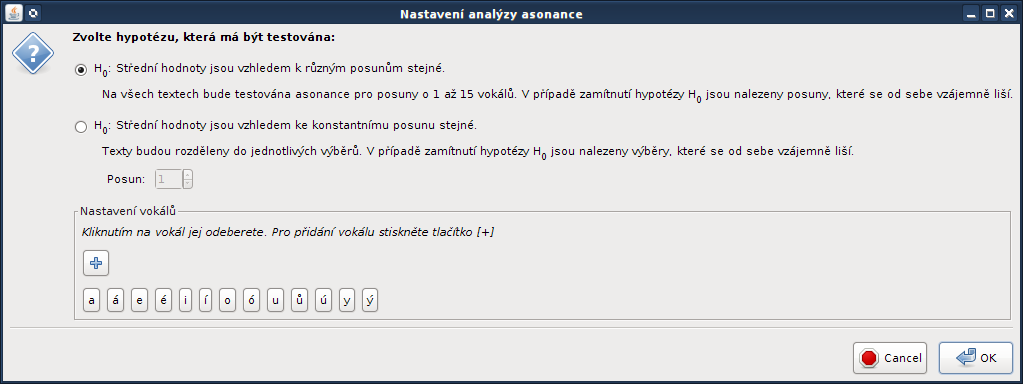
\includegraphics[max width=\textwidth,keepaspectratio=true]{imgs-60-aplikace/gui-asonance-settings}
\caption{Nastavení asonance.}
\label{fig:gui-asonance-settings}
\end{figure}

V rámci asonance je možné testovat dvě rozdílné hypotézy $H_0$:
\begin{description}
\item[Střední hodnoty jsou vzhledem k různým posunům stejné] Na všech textech je provedena asonance pro posuny o jeden až patnáct vokálů. Testované skupiny jsou vytvořeny automaticky -- co posun, to skupina. V případě zamítnutí nulové hypotézy jsou nalezeny posuny, které se od sebe významně liší. 

\item[Střední hodnoty jsou vzhledem ke konstantnímu posunu stejné] Nejprve je zvolen posun, pro nějž bude testována shoda středních hodnot. V dalším kroku je třeba texty rozdělit do jednotlivých skupin. Lze tak porovnat asonance například u různých autorů či jazyků. K~rozdělení otevřených textů do skupin slouží dialog, který je otevřen po kliknutí na tlačítko \keys{OK} v dialogu nastavení asonance:
\begin{figure}[H]
\centering
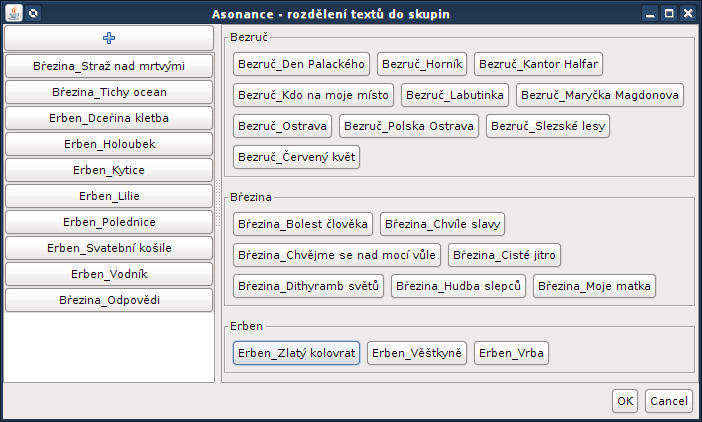
\includegraphics[max width=\textwidth,keepaspectratio=true]{imgs-60-aplikace/gui-asonance-settings-groups}
\caption{Nastavení asonance -- dělení textů do skupin.}
\label{fig:gui-asonance-settings-groups}
\end{figure}

\end{description}


\subsection{Denotační analýza}
\label{chap:app-denotation-analysis}
Denotační analýza je prováděna vždy pouze na jednom (aktivním) textu. Je možné ji vyvolat dvěma způsoby:

\begin{enumerate}
\item v menu aplikace \menu[,]{Analýza,Denotační analýza},
\item v panelu nástrojů zvolit \menu[,]{Analýza jednoho textu,Denotační analýza}.
\\
\end{enumerate}

Po zvolení jedné z možností se otevře nové okno. Jak bylo popsáno v kapitole \hyperref[chap:denotacni_analyza]{Denotační analýza}, je třeba nejprve zkoumaný text rozdělit do hřebů. K tomuto účelu slouží právě nově otevřené okno:
\begin{figure}[H]
\centering
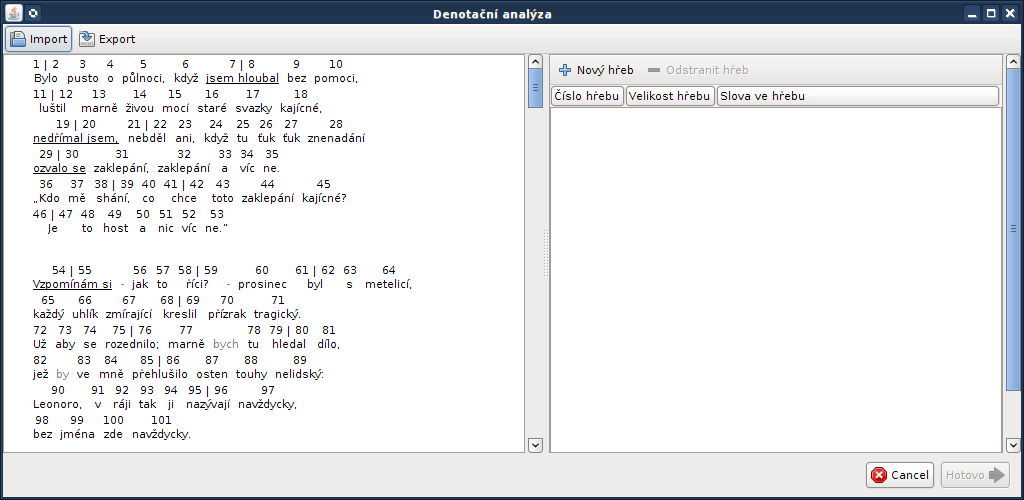
\includegraphics[max width=\textwidth,keepaspectratio=true]{imgs-60-aplikace/gui-denotation-window}
\caption{Okno pro dělení textu do hřebů.}
\label{fig:gui-denotation-window}
\end{figure}

Na horním okraji okna je umístěn nástrojový panel, který obsahuje tlačítka pro nahrání dříve uloženého rozdělení textu (tlačítko \keys{Import}) a tlačítko \keys{Export} pro uložení rozpracovaného rozdělení. 

Prostřední část okna je rozdělena na dva sloupce, z nichž levý obsahuje analyzovaný text včetně očíslovaných denotačních elementů a v pravém sloupci je umístěna tabulka s vytvořenými hřeby (na obrázku \ref{fig:gui-denotation-window} nejsou zatím žádné hřeby vytvořeny). Nad tabulkou se nachází tlačítka pro vytvoření nového hřebu a smazání vybraného hřebu. 

V pravém dolním rohu se nachází tlačítka \keys{Cancel} a \keys{Hotovo}. Tlačítkem \keys{Cancel} je možné zavřít okno pro dělení textu (přitom je uživatel upozorněn, že zavřením okna přijde o rozdělanou práci a je mu nabídnuta možnost rozpracované rozdělení uložit). Tlačítko \keys{Hotovo} je neaktivní, dokud nejsou všechny denotační elementy roztříděny do hřebů. Po kliknutí na něj je zobrazen dialog, ve kterém uživatel může hotové rozdělení uložit (aby jej příště mohl opět otevřít a použít). Nakonec je okno pro dělení textu do hřebů uzavřeno a místo něj se zobrazí okno s~výsledky denotační analýzy na základě vytvořeného rozdělení.

\subsubsection{Dělení do hřebů}

Rozdělení slov do hřebů se program snaží co možná nejvíce usnadnit. Správa hřebů je soustředěna do pravé části okna. Po spuštění je tato oblast prázdná, neboť zatím nebyl vytvořen žádný hřeb. Nový hřeb se vytvoří kliknutím na tlačítko \keys{Nový hřeb}. Nově vytvořený hřeb je zobrazen jako řádek v tabulce. Kliknutím na právě vytvořený hřeb se hřeb označí a aktivuje se tlačítko \keys{Odstranit hřeb}. Po kliknutí na něj jsou ze hřebu odstraněny všechny denotační elementy a hřeb je smazán.

Levá část okna obsahuje text analyzované básně, který je doplněn o čísla denotačních elementů. Manipulace s denotačními elementy probíhá přes kontextové menu, které je vyvoláno kliknutím pravým tlačítkem myši na příslušné slovo básně.

\begin{figure}[H]
\centering
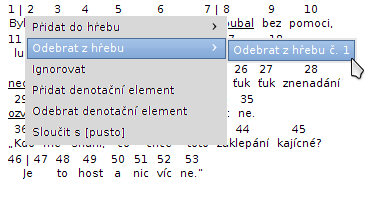
\includegraphics[max width=\textwidth,keepaspectratio=true]{imgs-60-aplikace/gui-denotation-element-menu}
\caption{Kontextové menu denotačního elementu \enquote{Bylo}.}
\label{fig:gui-denotation-menu}
\end{figure}

Kontextové menu obsahuje různý počet položek v závislosti na aktuálním stavu daného slova. 

\begin{description}[style=nextline]
	\item[\keys{Přidat do hřebu $\kern 10pt\triangleright$}] Tato volba je zobrazena pouze v případě, že již byl vytvořen alespoň jeden hřeb. Obsahuje podmenu, v němž je možné zvolit hřeb, do nějž má být denotační element přidán. Denotační elementy jsou kvůli přehlednosti rozděleny do skupin po dvaceti.

	\item[\keys{Přidat do jiného hřebu}] Tato volba je viditelná pouze, pokud již byly všechny denotační elementy daného slova zařazeny do hřebů a současně existuje hřeb, v němž se žádný z denotačních elementů tohoto slova nenachází (tzn. bylo vytvořeno více hřebů, než má dané slovo elementů). Touto volbou je možné zařazení jednoho denotačního elementu do více hřebů.

	\item[\keys{Odebrat z hřebu $\kern 10pt\triangleright$}] Volba je viditelná pouze u slov, která již byla přidána do nějakého hřebu. Pomocí této volby je možné denotační element z hřebu odstranit. V podmenu jsou zobrazeny všechny hřeby, do nichž byly denotační elementy zvoleného slova zařazeny. Kliknutím na položku je příslušný element odstraněn z vybraného hřebu.

	\item[\keys{Ignorovat} / \keys{Brát v potaz}] Tyto dvě volby umožňují dané slovo vyřadit z analýzy (případně zařadit zpět). Ignorovaná slova jsou v textu zašedlá a nejsou nad nimi zobrazena čísla denotačních elementů. Volby \keys{Ignorovat} a \keys{Brát v potaz} jsou zobrazeny v závislosti na tom, zda je dané slovo  ignorováno, či nikoliv.

	\item[\keys{Přidat denotační element}] Tato volba přidá k danému slovu nový denotační element, jehož číslo bude o jedna vyšší, než nejvyšší číslo z elementů, které již jsou slovu přiřazeny. 

	\item[\keys{Odebrat denotační element}] Tato volba je dostupná pouze pro slova, která mají alespoň dva denotační elementy. Použitím této volby je denotační element s nejvyšším číslem smazán.

	\item[\keys{Sloučit s [\ldots]}] Tato volba umožňuje z více slov vytvořit jeden denotační element (např. složená slovesa jako \enquote{nedřímal jsem}). K dispozici je vždy sloučení s následujícím slovem, což v některých případech nemusí vyhovovat. Například na obrázku \ref{fig:gui-denotation-window} je v devátém verši

		\begin{verse}
		\enquote{Už aby se rozednilo; marně bych tu hledal dílo,\ldots}
		\begin{flushright}
		\textit{(Havran --- překlad Ivan Slavík)}
		\end{flushright}
		\end{verse}

	složené sloveso \enquote{hledal bych}. V tomto případě program nabídne sloučení \enquote{bych} se slovem \enquote{tu}, což není požadovaný výsledek. Řešením je proto slovo \enquote{bych} ignorovat a \mbox{chovat} se, jako by se o složené sloveso nejednalo (jak je vidět i na obrázku \ref{fig:gui-denotation-window}). Obdobná situace nastala i ve verši desátém.
\end{description}

Pomocí kontextového menu je třeba rozdělit do hřebů všechny denotační elementy, které jsou v básni vytvořeny. Dokud není každý denotační element zařazen do hřebu, nedovolí aplikace pokračovat. Výhodné je průběžně ukládat stav rozdělování, aplikace sama rozdělanou práci periodicky neukládá.

Poté, co je rozdělování dokončeno, je zpřístupněno tlačítko \keys{Hotovo}. Kliknutím na něj se okno s dělením uzavře a otevře se okno s výsledky denotační analýzy. Jako první jsou zobrazeny souhrnné informace jako kompaktnost textu $K$, centralizovanost textu $R$ a hodnota MacIntoshova indexu.

Analýza dále obsahuje sekci, v níž je zobrazena difuze hřebů a poziční hřeby. Tyto sekce jsou ve výchozím stavu sbaleny.

Níže je zobrazena sekce \enquote{Jádro textu}. Aplikace sama vytvořila jádro textu ze hřebů, které obsahují alespoň dva denotační elementy. Pokud některý z vybraných hřebů do jádra textu nepatří, je možné jej z jádra odstranit kliknutím na něj levým tlačítkem myši. Tím se hřeb přesune do podsekce \enquote{Hřeby mimo jádro}. V případě, že by do jádra patřil hřeb nacházející se v~podsekci \enquote{Hřeby mimo jádro}, lze ho jej mezi jaderné hřeby zařadit opět kliknutím levým tlačítkem myši. Poslední podsekce je \enquote{Tematičnost jádrových hřebů}, v níž je pro každý jádrový hřeb zobrazena jeho tematičnost. 

Další sekcí je sekce \enquote{Rozšířené jádro textu}. V té jsou na základě vytvořeného jádra textu zobrazeny hřeby patřící do rozšířeného jádra.

Výsledný report denotační analýzy uzavírají sekce týkající se grafů --- \enquote{Koincidence} a \enquote{Graf}. Aplikace pracuje s rámcem koincidence stanoveným jako verš. Sekce \enquote{Koincidence} zahrnuje dvě podsekce:
\begin{enumerate}
\item \enquote{Báseň jako pořadová čísla hřebů} obsahuje přepis básně, kde jsou namísto slov zobrazena pořadová čísla hřebů. 
\item \enquote{Tabulka koincdence} zobrazuje v tabulce koincidence pro všechny páry veršů. Nad tabulkou je umístěn výběr základního verše.
\end{enumerate}

Poslední sekcí je sekce \enquote{Graf}. V té se, jak název napovídá, nachází graf. Ve výchozím stavu je graf sestaven na základě vypočítaných koincidencí a zvolené kritické hodnoty $\alpha$. Výchozí hodnota $\alpha = 0,1$. Kritickou hodnotu je možné měnit v ovládacím panelu nad grafem. 

Typ grafu je možné změnit z koincidenčního na deterministicko-pravděpodobností. K tomu slouží tlačítka \keys{Graf koincidence} a \keys{Deterministický graf} nacházející se pod volbou kritické hodnoty $\alpha$. 

Panel dále obsahuje zaškrtávací volbu \enquote{Povolit automatické rozmístění grafu}. Je-li automatické rozmístění povoleno, jsou vrcholy grafu rozmístěny automaticky tak, aby se hrany co nejméně překrývaly. Protože výsledky automatického rozmístění nebývají stoprocentní, je vhodné volbu povolit při změně kritické hodnoty $\alpha$, poté zakázat a rozmístění vrcholů dokončit ručně. Při povolení funkce jsou vrcholy vždy rozmístěny znovu.

Třetí a poslední funkcionalita, kterou panel nabízí, je uložení grafu do souboru PNG.

\section{Implementace denotační analýzy}

Implementace denotační analýzy byla největším a nejtěžším úkolem, který byl během vývoje aplikace realizován. Denotační analýza sestává ze dvou částí:
\begin{itemize}
\item dělení textu do hřebů,
\item zobrazení výsledků denotační analýzy včetně grafu.
\end{itemize}

I když to nemusí být na první pohled zřejmé, implementace dělení textu do hřebů si \mbox{vyžádala} delší čas a byla náročnější než implementace části druhé. Při dělení textu jsou využívány dvě poměrně komplexní datové struktury (DS), které budou ještě později podrobně popsány. První je uživateli graficky zobrazena v levé části okna a představuje analyzovaný text s jednotlivými denotačními elementy. Druhá reprezentuje jednotlivé etablované hřeby včetně \mbox{denotačních} elementů, které byly do daného hřebu zařazeny. 

Obě tyto struktury navíc umožňují serializaci a deserializaci do/ze souboru. Implementována byla serializace do textového souboru do formátu vycházejícího z \acrshort{csv}. Výhodou tohoto řešení je, že uživatel může nezávisle na aplikaci soubor otevřít a upravit. Při vývoji aplikace (ale i při realizaci praktické části této práce) přišla tato vlastnost vhod, neboť se nejednou stalo, že data byla vyexportována tak, že nemohla být opětovně načtena. Ručním zásahem se podařilo uložený soubor opravit a tak zachránit rozdělanou práci.

V následujícím textu budou popsány implementační detaily denotační analýzy z pohledu datových struktur. Vytváření grafického uživatelského rozhraní na základě těchto datových struktur prezentováno nebude. Popsané datové struktury jsou implementovány jak v knihovně \texttt{compLing}, tak v modulu grafického uživatelského rozhraní. V tom byly rozšířeny zejména o funkce nutné ke grafické reprezentaci. Příloha \ref{appendix:class-diagram} obsahuje \acrshort{uml} diagramy tříd denotační analýzy jak v modulu uživatelského rozhraní, tak v knihovně \texttt{compLing}.

\subsection{Implementace v knihovně \texttt{compLing}}

Objekt zapouzdřující v knihovně \texttt{compLing} denotační analýzu je typu \texttt{IDenotation}, což je rozhraní (interface). To přináší výhodu v tom, že by jeho implementace mohla být snadno změněna bez vlivu na ostatní části programu. Rozhraní \texttt{IDenotation} je včetně své implementace třídou \texttt{Denotation} zobrazeno formou třídního diagramu v příloze \ref{appendix:class-diagram} na obrázku \ref{fig:gui-idenotation-class-diagram}. Diagram tříd níže popsaných datových struktur je možné si prohlédnout taktéž v příloze \ref{appendix:class-diagram} na obrázku \ref{fig:compling-denotation-class-diagram}.

Třída \texttt{Denotation} implementuje metody definované rozhraním \texttt{IDenotation}. Do jejího konstruktoru je argumentem předána analyzovaná báseň typu \texttt{Poem}. Na jejím základě je vytvořena \texttt{DenotationPoem}. Ta obsahuje kolekci slov analyzované básně (\texttt{DenotationWord}). 

Třída \texttt{Denotation} dále obsahuje referenci na třídu type \texttt{HrebsHolder}, což je třída zodpovědná za práci s etablovanými hřeby. Hřeby (představované třídou \texttt{Hreb}) jsou drženy v kolekci typu tabulka. Jejím klíčem je číslo představující identifikátor hřebu. Hodnotou je pak konkrétní instance třídy \texttt{Hreb}. \texttt{HrebsHolder} si navíc udržuje nejvyšší číslo doposud vytvořeného hřebu, které je použito při vytváření hřebu nového.

Výpočty spojené s denotační analýzou jsou implementovány třídou \texttt{DenotationMath}. Tato třída neobsahuje žádné vlastnosti, jsou do ní soustředěny pouze metody pro \mbox{výpočty} kompaktnosti, centralizovanosti, MacInthoshova indexu, indexů nespojitosti a neizolovanosti,~\ldots Výpočet indexu dosažitelnosti je oproti jiným výpočtům komplexnější, a proto jej má na starost vlastní třída \texttt{ReachabilityIndexMath}.

U každého slova \texttt{DenotationWord} jsou kromě slova samotného uloženy i informace o jeho pořadí v básni, dále číslo verše a strofy, v nichž se v básni nachází. \texttt{DenotationWord} dále obsahuje dva seznamy:
\begin{itemize}
\item Seznam \texttt{joinedWords}, v němž jsou uložena slova, se kterými je dané slovo spojeno pomocí volby \keys{Sloučit s [\ldots]}. Je-li tento seznam prázdný, není slovo spojeno se žádným jiným slovem.
\item Seznam \texttt{denotationElements} obsahující denotační elementy daného slova. Jejich počet je ovlivnitelný volbami \keys{Přidat denotační element} a \keys{Odebrat denotační element}. Na začátku analýzy je každému slovu přiřazen právě jeden denotační element.
\end{itemize}

Slovo může být v z denotační analýzy vynecháno. Informace o tom, zda je konkrétní \texttt{DenotationWord} ignorováno, je držena v proměnné \texttt{ignored} typu \texttt{boolean}. Pro každé slovo je také držena informace o tom, zda je samo spojeno s nějakým jiným slovem (tzn., zda se nachází v seznamu \texttt{joinedWords} některého jiného slova). Tato informace je držena v proměnné typu \texttt{boolean} pojmenované \texttt{joined}.

Třída \texttt{Hreb} uchovává číslo hřebu a množinu slov (\texttt{DenotationWord}), která byla do daného hřebu zařazena. Číslo hřebu může být pouze sníženo, a to v případě, že je smazán hřeb s nižším číslem. Ke zvýšení čísla hřebu dojít nemůže, neboť třída \texttt{HrebsHolder} zajišťuje, že číslo nového hřebu je vyšší než číslo všech existujících hřebů.

Informaci o tom, který denotační element patří do kterého hřebu, nese třída \texttt{DenotationElement}. Na začátku analýzy je každému slovu (\texttt{DenotationWord}) přiřazen jeden denotační element. Každý objekt \texttt{DenotationElement} je pevně spojen s jedním slovem. Dále je u každého denotačního elementu uloženo jeho číslo, hřeb, do kterého je denotační element zařazen (může být i \texttt{null}, pokud do žádného hřebu zařazen není). Pokud do hřebu patří pouze část denotačního elementu, je tato informace také uložena.

\subsection{Implementace v modulu uživatelského rozhraní}

Datové struktury vytvořené v rámci modulu uživatelského grafického rozhraní rozšiřují výše popsané \acrshort{ds} knihovny \texttt{compLing} zejména o vlastnosti nutné k propojení s \acrshort{gui}. Jedná se typicky o zapouzdření (encapsulation) původní datové struktury do struktury nové.

Z hlediska hierarchie modulu grafického rozhraní je nejvýše postavenou třídou v rámci denotační analýzy třída \texttt{GuiDenotationAnalysis}. Ta je zodpovědná za propojení \acrshort{gui} s~datovým modelem (\acrshort{gui} $\leftrightarrow$ akce uživatele $\leftrightarrow$ datový model $\leftrightarrow$ \acrshort{gui}). Konstruktoru třídy \texttt{GuiDenotationAnalysis} je předán pracovní text (\texttt{WorkingText}). Na jeho základě je vytvořen datový model denotační analýzy:

Základ \acrshort{ds} denotační analýzy tvoří třída \texttt{GuiDenotationModel}, která implementuje  rozhraní \texttt{Csv<GuiDenotationModel>}. Rozhraní \texttt{Csv<T>} je generické a definuje metody potřebné pro uložení a načtení objektu typu \texttt{T} z, resp. do, souboru. Kromě toho \texttt{GuiDenotationModel} obsahuje reference na dvě další datové struktury: 
\begin{itemize}
\item \texttt{GuiDenotationPoemModel}, který představuje analyzovaný text a v něm vytvořené denotační elementy;
\item \texttt{GuiDenotationSpikesModel} reprezentující etablované hřeby a do nich zařazené denotační elementy.
\end{itemize}

Obě dvě tyto třídy implementují rozhraní \texttt{Csv}, díky kterému mohou být uloženy do souboru.

Třída \texttt{GuiDenotationAnalysis} dále obsahuje kolekci \texttt{GuiDenotationWord}. Třída \texttt{GuiDenotationWord} zapouzdřuje objekt \texttt{DenotationWord} a poskytuje metody, které jsou volány z kontextového menu jednotlivých slov analyzovaného textu (viz \ref{chap:app-denotation-analysis}).

\end{document}